\documentclass[12pt, a4paper]{ntut-report}
\usepackage[dvips,xetex]{graphicx}
\usepackage{ifpdf,mla}% <-- mla.sty requires ifpdf.sty, but (perversely) doesn't load it
%\usepackage{fontspec}
\usepackage{geometry}
\usepackage{lipsum}
\usepackage{xeCJK}
\usepackage{wallpaper}
\usepackage{pdfpages}
\usepackage{indentfirst}
\usepackage{setspace}
\usepackage{hyperref}
\usepackage{zhnumber}
\usepackage{titlesec}
\usepackage{amsmath}
\usepackage[backend=bibtex,sorting=none]{biblatex}

%
% this file is encoded in utf-8
%

% %%%%%%%%%%%%%%%%%%%%%%%%%%%%%%%%%%%%%%%%%%%%%%%%%%
% Configs
% %%%%%%%%%%%%%%%%%%%%%%%%%%%%%%%%%%%%%%%%%%%%%%%%%%

% studentDegree = master | doctor
\newcommand\studentDegree{master}

% platformFont = overleaf | windows | linux (TODO) | macOs (TODO)
\newcommand\platformFont{windows}

% ntutThesisLanguage = en | zh-tw
\newcommand\ntutThesisLanguage{zh-tw}

% ntutThesisPurpose = paperCopies | upload
\newcommand\ntutThesisPurpose{paperCopies}

% %%%%%%%%%%%%%%%%%%%%%%%%%%%%%%%%%%%%%%%%%%%%%%%%%%
% Labels
% %%%%%%%%%%%%%%%%%%%%%%%%%%%%%%%%%%%%%%%%%%%%%%%%%%

% Thesis Title
\newcommand\thieseTitleZhTw{基於沙盒系統之程式評測應用}
\newcommand\thieseTitleEn{Online Judge System based on Sandbox System}

% Student Name
\newcommand\studentNameZhTw{黃漢軒}
\newcommand\studentNameEn{Huang, Han-Xuan}

% Advisor
\newcommand\advisorNameZhTw{郭忠義 博士}
\newcommand\advisorNameEn{Dr. Kuo Jong-Yi}

% University Name
\newcommand\universityNameZhTw{國立臺北科技大學}
\newcommand\universityNameEn{National Taipei University of Technology}

% Department Name
\newcommand\departmentNameZhTw{資訊工程系}
\newcommand\departmentNameEn{Department of Computer Science and Information Engineering}

% Oral Defense Date (ISO8601) (yyyy-mm-dd)
\newcommand\oralDefenseDate{2025-05-01}

% %%%%%%%%%%%%%%%%%%%%%%%%%%%%%%%%%%%%%%%%%%%%%%%%%%
% English abstract content
% 英文摘要內容
\newcommand\abstractDescriptionContentEn{
    Start writing abstract from here.
    Start writing abstract from here.
    Start writing abstract from here.
    Start writing abstract from here.

    Start writing abstract from here.
    Start writing abstract from here.
    Start writing abstract from here.
    Start writing abstract from here.\\
    Start writing abstract from here.
    Start writing abstract from here.
    Start writing abstract from here.
    Start writing abstract from here.
}
% Keywords – please fill in yourself. Separate multiple keywords with commas (,).
\newcommand\keywordEn{
    LaTeX, 
    Thesis
}

% %%%%%%%%%%%%%%%%%%%%%%%%%%%%%%%%%%%%%%%%%%%%%%%%%%
% Chinese abstract content
% This section can be skipped if you are writing your thesis in English.
% 
% 中文摘要內容
% 如果您使用英文撰寫論文,則可以跳過此部分。
\newcommand\abstractDescriptionContent{
    摘要為論文或報告的精簡概要,其目的是透過簡短的敘述使讀者大致瞭解整篇報告的內容。
    摘要的內容通常須包括問題的描述以及所得到的結果,但以不超過 500 字或一頁為原則,且不得有參考文獻或引用圖表等。
    以中文撰寫之論文除中文摘要外,得於中文摘要後另附英文摘要。
    標題使用 20pt 粗標楷體並於上、下方各空一行(1.5 倍行高,字型 12pt 空行)後鍵入摘要內容。
    摘要頁須編頁碼(小寫羅馬數字表示頁碼)。
}
% 關鍵詞,請自己填,多個關鍵字以逗號(、)隔開
\newcommand\keywordZhTw{
    LaTeX、
    論文
}

% %%%%%%%%%%%%%%%%%%%%%%%%%%%%%%%%%%%%%%%%%%%%%%%%%%
% Acknowledgments
% 致謝
\newcommand\acknowledgmentsContent{
    所有對於研究提供協助之人或機構,作者都可在誌謝中表達感謝之意。
}

% %%%%%%%%%%%%%%%%%%%%%%%%%%%%%%%%%%%%%%%%%%%%%%%%%%
% Basic Utils
% %%%%%%%%%%%%%%%%%%%%%%%%%%%%%%%%%%%%%%%%%%%%%%%%%%

\newcommand{\removeLeadingZero}[1]{%
  \ifnum#1<10 #1\else#1\fi
}

\newcommand{\mapNumToMonthTextEn}[1]{
  \ifcase#1\or January\or February\or March\or April\or May\or June\or July\or August\or September\or October\or November\or December\fi
}

% 中文數字轉換(0~9)
\newcommand{\mapNumToTextZhTw}[1]{%
  \ifcase#1 零\or 一\or 二\or 三\or 四\or 五\or 六\or 七\or 八\or 九\fi
}

% 阿拉伯數轉中文數字(支援 1~999)
\newcommand{\mapNumberToTextZhTw}[1]{%
  \ifnum#1<10
    \mapNumToTextZhTw{#1}%
  \else
    \ifnum#1<100
      \mapNumToTextZhTw{\numexpr#1/10\relax}十%
      \ifnum\numexpr#1-\numexpr(#1/10)*10\relax>0
        \mapNumToTextZhTw{\numexpr#1-\numexpr(#1/10)*10\relax}%
      \fi
    \else
      \mapNumToTextZhTw{\numexpr#1/100\relax}百%
      \ifnum\numexpr(#1/10)-(\numexpr#1/100)*10\relax>0
        \mapNumToTextZhTw{\numexpr(#1/10)-(\numexpr#1/100)*10\relax}十%
      \fi
      \ifnum\numexpr#1-\numexpr(#1/10)*10\relax>0
        \mapNumToTextZhTw{\numexpr#1-\numexpr(#1/10)*10\relax}%
      \fi
    \fi
  \fi
}

% ==================================================
% ISO 8601

\newcommand{\mapIsoDateToIsoYear}[1]{
  \begingroup
  \def\year{}%
  \def\processdate##1-##2-##3\@nil{%
    \def\year{##1}%
  }%
  \expandafter\processdate#1\@nil
  \year%
  \endgroup
}

\newcommand{\mapIsoDateToIsoMonth}[1]{
  \begingroup
  \def\month{}%
  \def\processdate##1-##2-##3\@nil{%
    \def\month{##2}%
  }%
  \expandafter\processdate#1\@nil
  \month%
  \endgroup
}

\newcommand{\mapIsoDateToIsoMonthTextEn}[1]{
  \begingroup
  \def\month{}%
  \def\processdate##1-##2-##3\@nil{%
    \def\month{##2}%
  }%
  \expandafter\processdate#1\@nil
  \mapNumToMonthTextEn\month%
  \endgroup
}

\newcommand{\mapIsoDateToIsoDay}[1]{
  \begingroup
  \def\day{}%
  \def\processdate##1-##2-##3\@nil{%
    \def\day{##3}%
  }%
  \expandafter\processdate#1\@nil
  \day%
  \endgroup
}

% ==================================================
% Anno Domini (AD)
\newcommand{\AdDate}[1]{%
  \begingroup
  \def\year{}%
  \def\month{}%
  \def\day{}%
  \def\processdate##1-##2-##3\@nil{%
    \def\year{##1}%
    \def\month{##2}%
    \def\day{##3}%
  }%
  \expandafter\processdate#1\@nil
  \mapNumToMonthTextEn{\month}\ \year%
  \endgroup
}

\newcommand{\AdDateWithComma}[1]{%
  \begingroup
  \def\year{}%
  \def\month{}%
  \def\day{}%
  \def\processdate##1-##2-##3\@nil{%
    \def\year{##1}%
    \def\month{##2}%
    \def\day{##3}%
  }%
  \expandafter\processdate#1\@nil
  \mapNumToMonthTextEn{\month}, \year%
  \endgroup
}

% ==================================================
% Republic of China (ROC)

% 主函數:輸出中華民國年+月(支援 \RocDate{yyyy-mm-dd})
\newcommand{\RocDate}[1]{%
  \begingroup
  \def\year{}%
  \def\month{}%
  \def\day{}%
  \def\processdate##1-##2-##3\@nil{%
    \def\year{##1}%
    \def\month{##2}%
    \def\day{##3}%
  }%
  \expandafter\processdate#1\@nil
  \def\ROCyear{\number\numexpr\year-1911\relax}%
  \def\ROCyearText{\mapNumberToTextZhTw{\ROCyear}}%
  中華民國\ROCyearText 年\mapNumberToTextZhTw{\month} 月%
  \endgroup
}

% %%%%%%%%%%%%%%%%%%%%%%%%%%%%%%%%%%%%%%%%%%%%%%%%%%
% Layouts
% %%%%%%%%%%%%%%%%%%%%%%%%%%%%%%%%%%%%%%%%%%%%%%%%%%

\renewcommand{\baselinestretch}{1.5}    % 將行距設為原來的 1.5 倍
\xeCJKsetup{
    AutoFakeBold=true,                  % 若所用中文字體不提供粗體版本,自動模擬出粗體效果。
    AutoFakeSlant=true,                 % 若所用中文字體不提供斜體版本,自動模擬出斜體效果。
}

% %%%%%%%%%%%%%%%%%%%%%%%%%%%%%%%%%%%%%%%%%%%%%%%%%%
% Customize fonts for cross-platform compatibility.
% 調整字體以實驗跨平台相容性

\ifthenelse{\equal{\platformFont}{overleaf}}{
    \setCJKmainfont{AR PL KaitiM Big5}      % 中文字體
    \setmainfont{Times New Roman}           % 英文字體
}

\ifthenelse{\equal{\platformFont}{windows}}{
    \setCJKmainfont{標楷體}                 % 中文字體
    \setmainfont{Times New Roman}           % 英文字體
}

\ifthenelse{\equal{\platformFont}{linux}}{
    % TODO
}

\ifthenelse{\equal{\platformFont}{macOs}}{
    % TODO
}

% %%%%%%%%%%%%%%%%%%%%%%%%%%%%%%%%%%%%%%%%%%%%%%%%%%
% 頁面設定,不需修改
\geometry{
    a4paper,
    total={297mm,210mm},
    top=4.5cm,
    bottom=0.75cm,
    left=2.5cm,
    right=2.2cm,
}

% %%%%%%%%%%%%%%%%%%%%%%%%%%%%%%%%%%%%%%%%%%%%%%%%%%
% Redefine commands for different NTUT thesis language
% %%%%%%%%%%%%%%%%%%%%%%%%%%%%%%%%%%%%%%%%%%%%%%%%%%

\ifthenelse{\equal{\ntutThesisLanguage}{en}}
{
  \renewcommand\acknowledgmentsName{Acknowledgments}
  \renewcommand\figureName{Figure}
  \renewcommand\tableName{Table}
  \renewcommand\tableOfContentsName{Table of Contents}
  \renewcommand\listOfFigureName{List of Figures}
  \renewcommand\listOfTableName{List of Tables}
  \renewcommand\referencesName{References}
}
{
  \renewcommand\acknowledgmentsName{誌謝}
  \renewcommand\figureName{圖}
  \renewcommand\tableName{表}
  \renewcommand\tableOfContentsName{目錄}
  \renewcommand\listOfFigureName{圖目錄}
  \renewcommand\listOfTableName{表目錄}
  \renewcommand\referencesName{參考文獻}
}


\pagestyle{plain} % 頁碼

\addbibresource{./bib/references.bib}      % 加入參考文獻檔案 reference.bib,用於 BibLaTeX 管理文獻
\graphicspath{{./assets/figures/}}  % 設定圖檔的預設路徑為 assets/figures 資料夾

% %%%%%%%%%%%%%%%%%%%%%%%%%%%%%%%%%%%%%%%%%%%%%%%%%%
% Contents
% %%%%%%%%%%%%%%%%%%%%%%%%%%%%%%%%%%%%%%%%%%%%%%%%%%

\begin{document}

% TODO
% --------------------------------------------------
% 
% I'm too lazy to use the .tex file for the book spine, 
% so please just use the Word template provided by the school to complete it.
% 
% --------------------------------------------------
% 
% 書背的 tex file 我懶得用,請直接用學校提供的 Word 模板完成
\ifthenelse{\equal{\ntutThesisPurpose}{paperCopies}}
{
    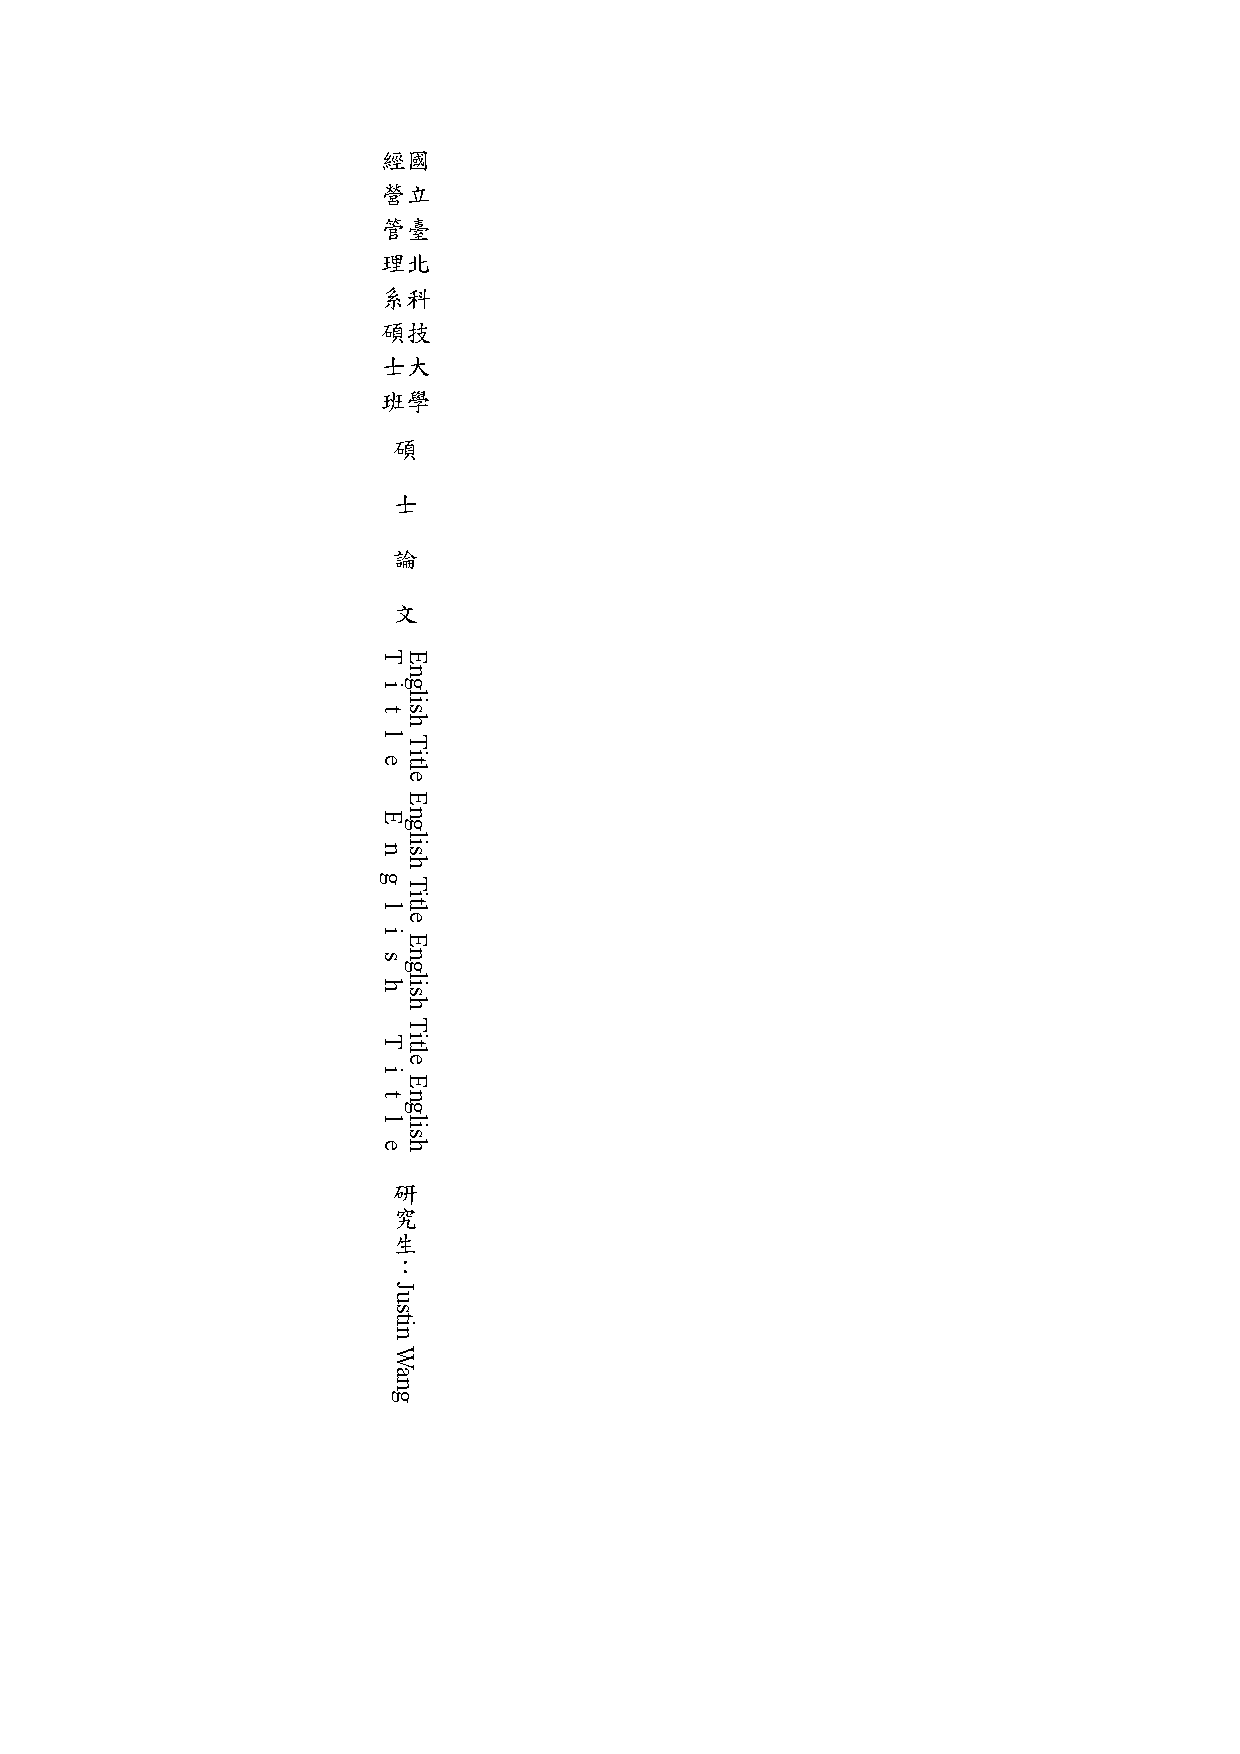
\includepdf[pages=-, trim=0mm 25.4mm 0mm -25.4mm]{static-page/spine.pdf}
}

% Cover without a watermark
% --------------------------------------------------
% 封面、不用浮水印
\ifthenelse{\equal{\ntutThesisPurpose}{paperCopies}}
{
    \pagenumbering{gobble}
\begin{titlepage}
    \newpage
    \begin{center}
        % 北科的 Logo
        
\includegraphics[width=13cm]{./logo/ntut-logo-with-label.png}
        
        % 北科的系所名與學位名,以換行隔開
        \huge\bf\departmentNameZhTw\ifthenelse{\equal{\studentDegree}{master}}{碩士}{博士}班\\
        \ifthenelse{\equal{\studentDegree}{master}}{
            \huge\bf 碩士學位論文\\% 學位名
        }{
            \huge\bf 博士學位論文\\% 學位名
        }
        \ifthenelse{\equal{\ntutThesisLanguage}{en}}{
            \Large\bf\departmentNameEn \\% 系所英文名
            \ifthenelse{\equal{\studentDegree}{master}}{
                \Large\bf Master Thesis\\% 學位名
            }{
                \Large\bf Ph.D. Dissertation\\% 學位名
            }
        }

        % 中文與英文論文名稱
        % 如果你不需要英文,你可以註解 \eTitle
        \vfill
        \huge\bf\thieseTitleZhTw\\ %%%%%
        \LARGE\bf\thieseTitleEn\\ %%%%%

        % 研究生(中文)
        \vfill
        {\Large 研究生:\studentNameZhTw}
        \ifthenelse{\equal{\ntutThesisLanguage}{en}}{
            \\{\Large Researcher: \studentNameEn}
        }

        % 指導老師(中文)
        \vfill
        {\Large 指導教授:\advisorNameZhTw}
        \ifthenelse{\equal{\ntutThesisLanguage}{en}}{
            \\{\Large Advisor: \advisorNameEn}
        }

        % 畢業年份(中文)
        \vfill
        {\Large \RocDate{\oralDefenseDate}}
        \ifthenelse{\equal{\ntutThesisLanguage}{en}}{
            \\{\Large \AdDate{\oralDefenseDate}}
        }
        
    \end{center}
\end{titlepage}
}

% Blank page without a watermark
% --------------------------------------------------
% 留白頁、不用浮水印
\ifthenelse{\equal{\ntutThesisPurpose}{paperCopies}}
{
    \clearpage
\thispagestyle{empty}
\null
\newpage
% (預留空白頁)
}

% Add Watermarks
% 新增浮水印
\CenterWallPaper{.64}{logo/ntut-logo.png}

% Cover with a watermark
% 封面、要浮水印
\pagenumbering{gobble}
\begin{titlepage}
    \newpage
    \begin{center}
        % 北科的 Logo
        
\includegraphics[width=13cm]{./logo/ntut-logo-with-label.png}
        
        % 北科的系所名與學位名,以換行隔開
        \huge\bf\departmentNameZhTw\ifthenelse{\equal{\studentDegree}{master}}{碩士}{博士}班\\
        \ifthenelse{\equal{\studentDegree}{master}}{
            \huge\bf 碩士學位論文\\% 學位名
        }{
            \huge\bf 博士學位論文\\% 學位名
        }
        \ifthenelse{\equal{\ntutThesisLanguage}{en}}{
            \Large\bf\departmentNameEn \\% 系所英文名
            \ifthenelse{\equal{\studentDegree}{master}}{
                \Large\bf Master Thesis\\% 學位名
            }{
                \Large\bf Ph.D. Dissertation\\% 學位名
            }
        }

        % 中文與英文論文名稱
        % 如果你不需要英文,你可以註解 \eTitle
        \vfill
        \huge\bf\thieseTitleZhTw\\ %%%%%
        \LARGE\bf\thieseTitleEn\\ %%%%%

        % 研究生(中文)
        \vfill
        {\Large 研究生:\studentNameZhTw}
        \ifthenelse{\equal{\ntutThesisLanguage}{en}}{
            \\{\Large Researcher: \studentNameEn}
        }

        % 指導老師(中文)
        \vfill
        {\Large 指導教授:\advisorNameZhTw}
        \ifthenelse{\equal{\ntutThesisLanguage}{en}}{
            \\{\Large Advisor: \advisorNameEn}
        }

        % 畢業年份(中文)
        \vfill
        {\Large \RocDate{\oralDefenseDate}}
        \ifthenelse{\equal{\ntutThesisLanguage}{en}}{
            \\{\Large \AdDate{\oralDefenseDate}}
        }
        
    \end{center}
\end{titlepage}

% Please add "Oral Defense Committee Signature Form" with complete signatures.
% 「學位論文口試委員會審定書」掃描檔,請檢附完整簽名之審定書掃描檔

\includepdf[pages=-, trim=0mm 25.4mm 0mm -25.4mm]{static-page/oral-defense-verification.pdf}

% Preface page numbers: lowercase Roman numerals.
% 前言頁碼:小寫羅馬數字
\pagenumbering{roman}

% Abstract (Chinese)
% 摘要頁(中文)
\ifthenelse{\equal{\ntutThesisLanguage}{zh-tw}}
{
    % 中文摘要頁
\begin{ZhAbstract}
    \begin{ZhAbstractItems}
    \noindent \text 關鍵詞:\keywordZhTw

    \end{ZhAbstractItems}

    \begin{ZhAbstractDescription}
        \abstractDescriptionContent
    \end{ZhAbstractDescription}
    
\end{ZhAbstract}
}

% Abstract (English)
% 摘要頁(英文)
% 英文摘要頁
\begin{EnAbstract}
    \begin{EnAbstractItems}
    \noindent \text Keyword: \keywordEn

    \end{EnAbstractItems}

    \begin{EnAbstractDescription}
        \abstractDescriptionContentEn
    \end{EnAbstractDescription}
    
\end{EnAbstract}

% Acknowledgements
% 致謝 
\begin{Acknowledgments}
    \acknowledgmentsContent
\end{Acknowledgments}

% Table of Contents, List of tables, List of figures
% 目錄、表目錄與圖目錄
\begin{TableOfContent}
    \tableOfContents
\end{TableOfContent}

\begin{TableOfContent}
    \listOfFigures
\end{TableOfContent}

\begin{TableOfContent}
    \listOfTables
\end{TableOfContent}
 
% Main text page numbers: Arabic numerals, starting again from page 1.
% 正文頁碼:阿拉伯數字,並重新編號為第 1 頁
\pagenumbering{arabic}

% Chapter 1
% 章節一
\begin{ZhChapter}

\chapter{緒論(大標)}

\section{研究動機與背景(小標)}

\begin{equation} 
    \mbox{$x = \dfrac{-b\pm\sqrt{b^2-4ac}}{2a}$}
\end{equation}

\subsection{研究背景(小小標)}

\text 背景內文背景內文背景內文背景內文,背景內文背景內文背景內文背景內文背景內文背景內文,如\cref{tab: table}所示,如\cref{tab: table,tab: complexity}所示,如\cref{fig: image}所示。

\begin{table*}[htbp]
    \centering
    \caption{表格範例標題} 
    \label{tab: table}
    \makebox[\linewidth][c]{
    \renewcommand\arraystretch{1.2}{
        \begin{tabular}{| l | c  c  c  c |}
        \hline
        Protocol & $P$ & $CS_1$ & $CS_2$ & $RG$ \\
        \hline
        SD & $O(1)$, $O(1)$, N/A & $O(n-t)$, $O(1)$, N/A & $O(n-t)$, $O(1)$, N/A & $O(1)$, $O(n)$, $O(n)$ \\
        MSSMul & $O(1)$, $O(1)$, N/A & $O(n-t)$, $O(n)$, $O(1)$ & $O(n-t)$, $O(n)$, N/A & $O(1)$, $O(n)$, $O(n)$ \\
        MSSAdd & $O(1)$, $O(1)$, N/A & $O(n-t)$, $O(n)$, $O(1)$ & N/A, N/A, N/A & $O(1)$, $O(n)$, $O(n)$ \\
        SC & $O(1)$, $O(1)$, N/A & $O(n-t)$, $O(n)$, $O(1)$ & $O(n-t)$, $O(n)$, N/A & $O(1)$, $O(n)$, $O(n)$ \\
        \hline 
        \end {tabular}
    }}
\end {table*}

\subsubsection{研究動機(小小標)}

\begin{equation} 
    \mbox{$(1+x)^n = 1 + \dfrac{nx}{1!} + \dfrac{n(n-1)x^2}{2!}$}
\end{equation}

動機動機動機動機,動機動機動機動機動機動機動機動機動機動機動機動機,動機動機動機動機動機動機動機動機。

動機動機動機動機動機動機動機動機,動機動機動機動機動機動機動機動機動機動機動機動機。動機動機動機動機動機動機動機動機,動機動機動機動機動機動機動機動機動機動機動機動機。動機動機動機動機動機動機動機動機,動機動機動機動機動機動機動機動機動機動機動機動機,如圖 1.1、圖 1.2 所示。

\begin{figure*}[htbp]
    \centering
    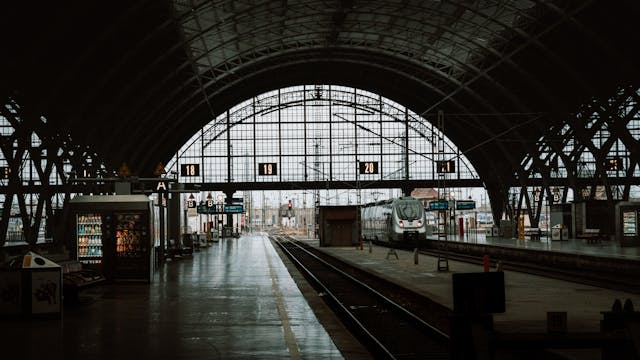
\includegraphics[width = 1\textwidth]{image.jpeg}
    \caption{Cool train station}
    \label{fig: image}
\end{figure*}

\begin{figure*}[htbp]
    \centering
    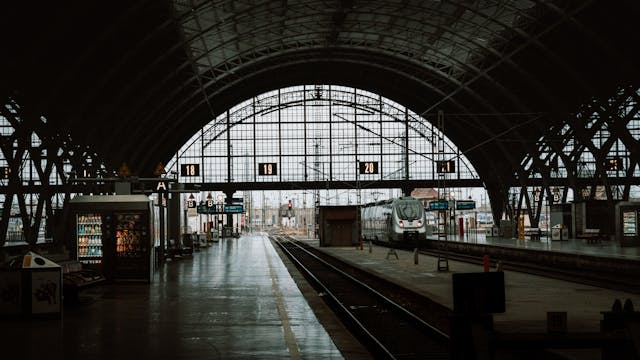
\includegraphics[width = 1\textwidth]{image.jpeg}
    \caption{Cool train station}
    \label{fig: image}
\end{figure*}

\begin{table*}[htbp]
    \centering
    \caption{表格範例標題} \label{tab: complexity}
    \makebox[\linewidth][c]{
    \renewcommand\arraystretch{1.2}{
        \begin{tabular}{| l | c  c  c  c |}
        \hline
        Protocol & $P$ & $CS_1$ & $CS_2$ & $RG$ \\
        \hline
        MSSMul & $O(1)$, $O(1)$, N/A & $O(n-t)$, $O(n)$, $O(1)$ & $O(n-t)$, $O(n)$, N/A & $O(1)$, $O(n)$, $O(n)$ \\
        MSSAdd & $O(1)$, $O(1)$, N/A & $O(n-t)$, $O(n)$, $O(1)$ & N/A, N/A, N/A & $O(1)$, $O(n)$, $O(n)$ \\
        SC & $O(1)$, $O(1)$, N/A & $O(n-t)$, $O(n)$, $O(1)$ & $O(n-t)$, $O(n)$, N/A & $O(1)$, $O(n)$, $O(n)$ \\
        MSSMul & $O(1)$, $O(1)$, N/A & $O(n-t)$, $O(n)$, $O(1)$ & $O(n-t)$, $O(n)$, N/A & $O(1)$, $O(n)$, $O(n)$ \\
        MSSAdd & $O(1)$, $O(1)$, N/A & $O(n-t)$, $O(n)$, $O(1)$ & N/A, N/A, N/A & $O(1)$, $O(n)$, $O(n)$ \\
        SC & $O(1)$, $O(1)$, N/A & $O(n-t)$, $O(n)$, $O(1)$ & $O(n-t)$, $O(n)$, N/A & $O(1)$, $O(n)$, $O(n)$ \\
        \hline 
        \end {tabular}
    }}
\end {table*}

動機動機動機動機,動機動機動機動機動機動機動機動機動機動機動機動機,動機動機動機動機動機動機動機動機。

動機動機動機動機,動機動機動機動機動機動機動機動機動機動機動機動機,動機動機動機動機動機動機動機動機。動機動機動機動機,動機動機動機動機動機動機動機動機動機動機動機動機,動機動機動機動機動機動機動機動機。

動機動機動機動機,動機動機動機動機動機動機動機動機動機動機動機動機,動機動機動機動機動機動機動機動機。動機動機動機動機,動機動機動機動機動機動機動機動機動機動機動機動機,動機動機動機動機動機動機動機動機。動機動機動機動機,動機動機動機動機動機動機動機動機動機動機動機動機,動機動機動機動機動機動機動機動機。

動機動機動機動機,動機動機動機動機動機動機動機動機動機動機動機動機,動機動機動機動機動機動機動機動機。動機動機動機動機,動機動機動機動機動機動機動機動機動機動機動機動機,動機動機動機動機動機動機動機動機。動機動機動機動機,動機動機動機動機動機動機動機動機動機動機動機動機,動機動機動機動機動機動機動機動機。動機動機動機動機,動機動機動機動機動機動機動機動機動機動機動機動機,動機動機動機動機動機動機動機動機。

\begin{figure*}[htbp]
    \centering
    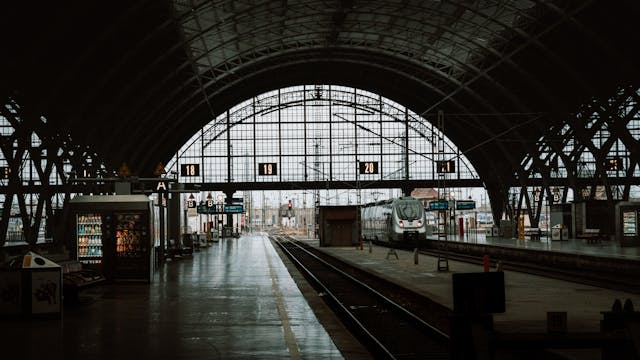
\includegraphics[width = 0.5\textwidth]{image.jpeg}
    \caption{Cool train station}
    \label{fig: image}
\end{figure*}

\end{ZhChapter}

% Chapter 2
% 章節二
\begin{ZhChapter}

\chapter{若標題太長,則可以分成兩行排列的形式撰寫}

\section{名詞定義(小標)}

定義定義定義定義定義定義\cite{latex2e},定義定義定義定義,定義定義定義定義定義定義定義定義定義定義,定義定義。

\begin{table*}[htbp]
    \centering
    \caption{表格範例標題} \label{tab: complexity}
    \makebox[\linewidth][c]{
    \renewcommand\arraystretch{1.2}{
        \begin{tabular}{| l | c  c  c  c |}
        \hline
        Protocol & $P$ & $CS_1$ & $CS_2$ & $RG$ \\
        \hline
        MSSMul & $O(1)$, $O(1)$, N/A & $O(n-t)$, $O(n)$, $O(1)$ & $O(n-t)$, $O(n)$, N/A & $O(1)$, $O(n)$, $O(n)$ \\
        SC & $O(1)$, $O(1)$, N/A & $O(n-t)$, $O(n)$, $O(1)$ & $O(n-t)$, $O(n)$, N/A & $O(1)$, $O(n)$, $O(n)$ \\
        \hline 
        \end {tabular}
    }}
\end {table*}

\section{模型說明(小標)}

說明說明說明說明,說明說明說明說明說明說明說明說明說明說明說明說明,說明說明說明說明說明說明說明說明。

\begin{figure*}[htbp]
    \centering
    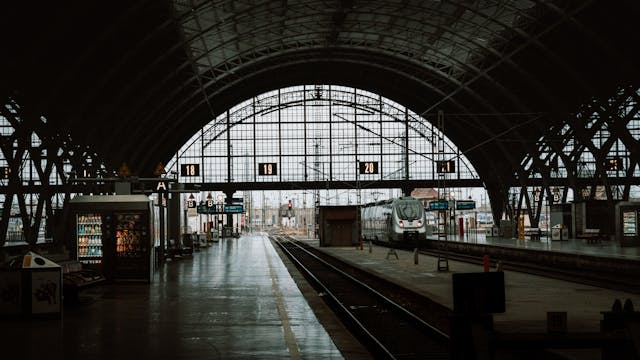
\includegraphics[width = 0.5\textwidth]{image.jpeg}
    \caption{Cool train station}
    \label{fig: image}
\end{figure*}

\begin{itemize}
    \item 主項目 A
    \begin{itemize}
        \item 子項目 A1
        \item 子項目 A2
    \end{itemize}
    \item 主項目 B
\end{itemize}

說明說明說明說明,說明說明說明說明說明說明說明說明說明說明說明說明,說明說明說明說明說明說明說明說明。

\begin{itemize}[label=--] % 將圓點改為破折號
    \item 自定義 bullet 1
    \item 自定義 bullet 2
\end{itemize}

\end{ZhChapter}

% Add chapters here...
% 新增你自己的章節...


% Please insert citations within the paragraphs as appropriate. 
% Ensure that the reference.bib file is included for proper reference management.
% 
% 參考文獻,請在段落上隨意註解,你同時需要 reference.bib
\addcontentsline{toc}{chapter}{參考文獻}
\printbibliography[title=參考文獻]


\end{document}
